\documentclass{beamer}

\usetheme{Madrid}

\usepackage{graphicx}
\usepackage{booktabs}
\usepackage{amsmath}
\usepackage{hyperref}
\usepackage{multicol}

\title{Analyzing the Impact of Random Factors on Student Performance}
\author{Derek}
\institute{}
\date{\today}

\begin{document}

\begin{frame}
  \titlepage
\end{frame}

\begin{frame}{Table of Contents}
  \begin{multicols}{2}
    \begin{itemize}
        \item Introduction
        \item Visuals: Introduction
        \item Background Information
        \item Research Questions
        \item Visuals: Research Questions
        \item Data Overview
        \item Visuals: Data Overview
        \item Preprocessing
        \item Visuals: Preprocessing
        \item Model
        \item Visuals: Model
        \item Results
        \item Visuals: Results
        \item Interpreting the Results
        \item Visuals: Interpreting the Results
        \item Model Evaluation
        \item Visuals: Model Evaluation
        \item Random Forest Evaluation
        \item Visuals: Random Forest Evaluation
        \item Analysis of the Results
        \item Visuals: Analysis of the Results
        \item Limitations
        \item Conclusion
        \item Next Steps
        \item Sources
        \item Acknowledgments
    \end{itemize}
  \end{multicols}
\end{frame}

\begin{frame}{Introduction}
  This presentation explores how demographic and behavioral factors affect student test scores. The dataset includes features such as gender, race/ethnicity, parental education, lunch type, and whether the student completed a test preparation course. The target variables are the math, reading, and writing scores, each ranging from 0 to 100.
\end{frame}

\begin{frame}{Background Information}
  The data is sourced from a public Kaggle dataset and simulates real-world standardized test outcomes. It contains a mix of categorical and numerical variables and provides a useful basis for exploring predictive modeling and educational insights.
\end{frame}

\begin{frame}{Research Questions}
  Our project addresses three main research questions:
  \begin{itemize}
    \item Does test preparation significantly improve math scores?
    \item What features are the most predictive of performance?
    \item Can a linear regression model adequately capture the trends in the data?
  \end{itemize}
\end{frame}

\begin{frame}{Visuals: Research Questions}
  \begin{figure}
    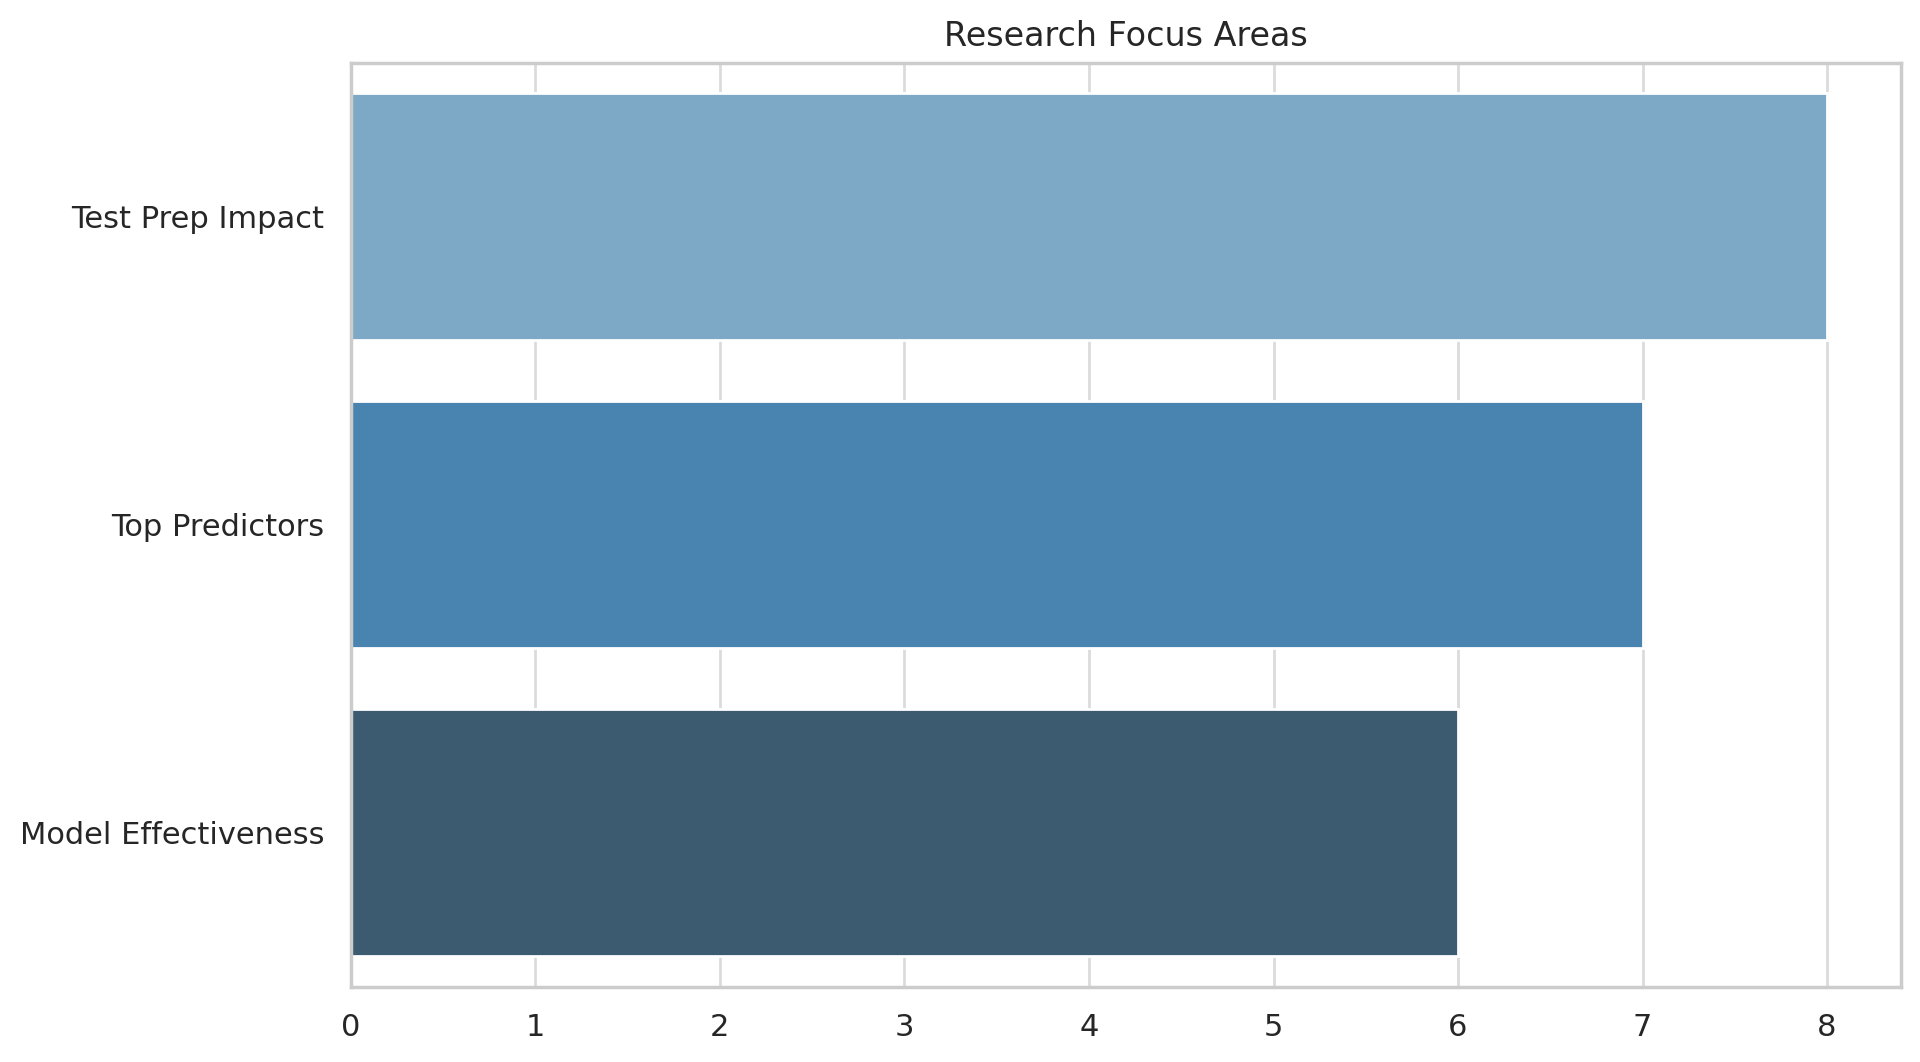
\includegraphics[width=0.9\linewidth]{research_questions_chart.png}
    \caption{Visual breakdown of research focus areas}
  \end{figure}
\end{frame}

\begin{frame}{Data Overview}
  The dataset includes over 1000 rows and 8 columns. Five are categorical variables: gender, race/ethnicity, parental education level, lunch type, and test preparation status. The remaining three are numeric: math score, reading score, and writing score.
\end{frame}

\begin{frame}{Visuals: Data Overview}
  \begin{figure}
    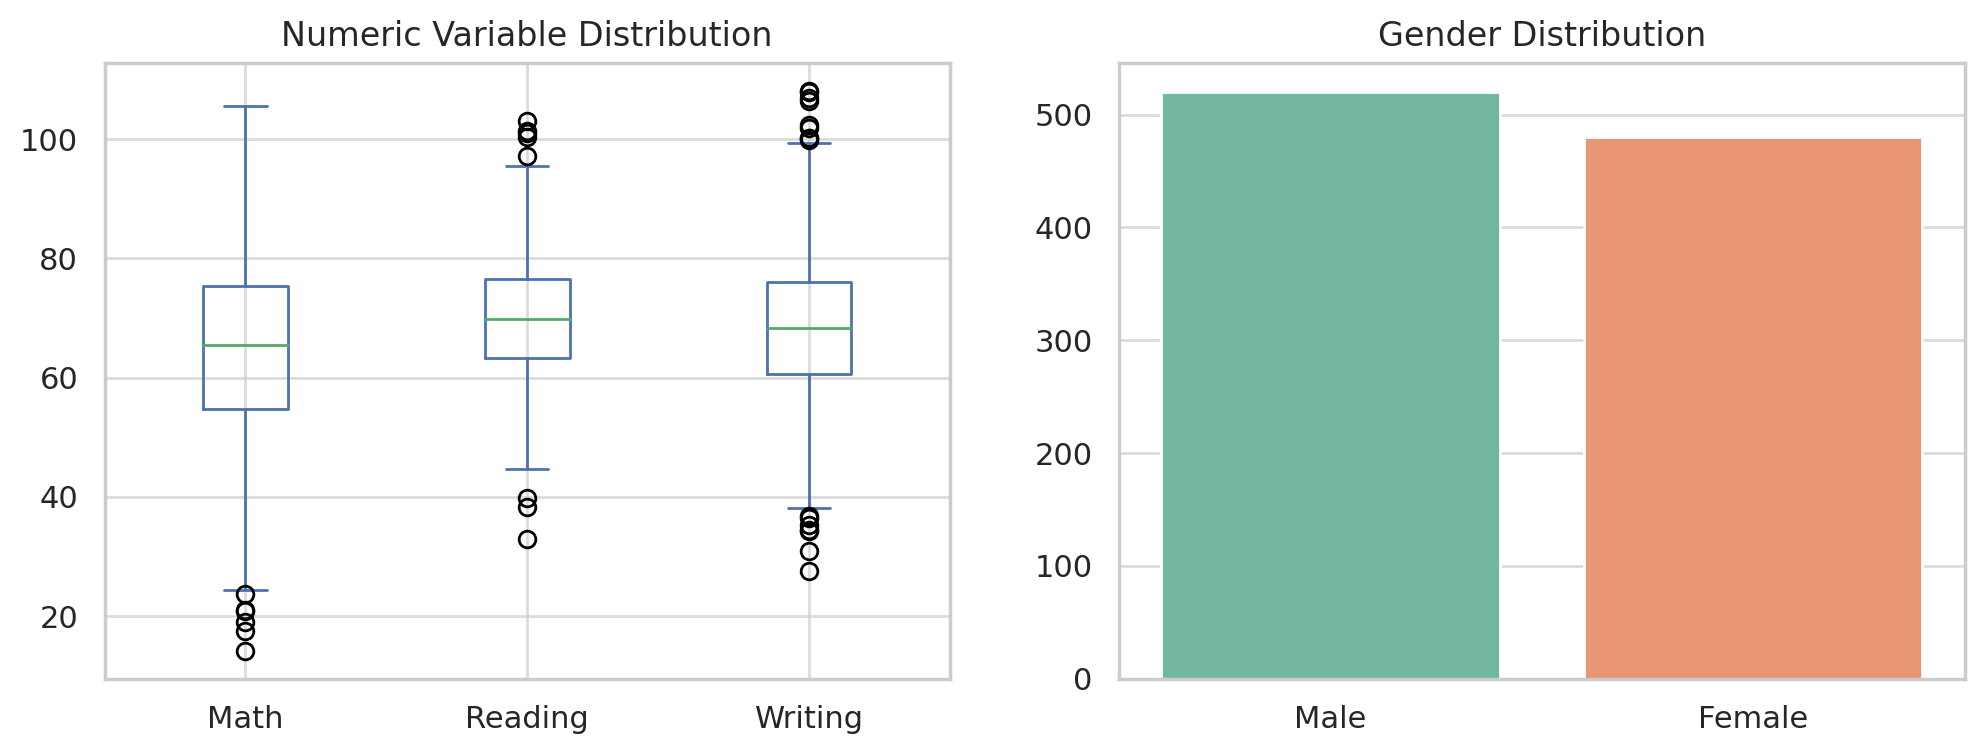
\includegraphics[width=0.9\linewidth]{data_distribution.png}
    \caption{Distribution of categorical and numeric variables}
  \end{figure}
\end{frame}

\begin{frame}{Preprocessing}
  We began by encoding the categorical variables. Binary categories such as gender were manually mapped (e.g., male = 1, female = 0). More complex categorical variables such as race and parental education were one-hot encoded. Finally, the dataset was split into training and testing sets using an 80\%--20\% split.
\end{frame}

\begin{frame}{Visuals: Preprocessing}
  \begin{figure}
    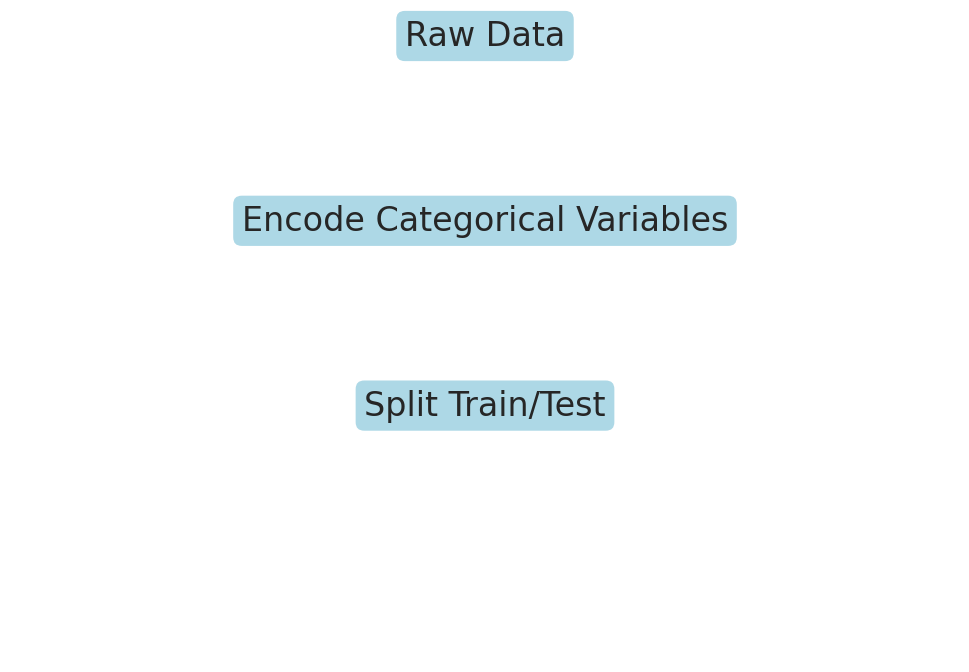
\includegraphics[width=0.9\linewidth]{preprocessing_pipeline.png}
    \caption{Preprocessing steps overview}
  \end{figure}
\end{frame}

\begin{frame}{Model}
  We used Linear Regression to predict math scores based on the provided features. The mathematical formula is:
  \[
  y = \beta_0 + \beta_1 x_1 + \beta_2 x_2 + \cdots + \beta_n x_n
  \]
  where \( y \) is the predicted math score, \( \beta_0 \) is the intercept, and \( \beta_1 \ldots \beta_n \) are the coefficients corresponding to the features \( x_1 \ldots x_n \).
\end{frame}

\begin{frame}{Visuals: Model}
  \begin{figure}
    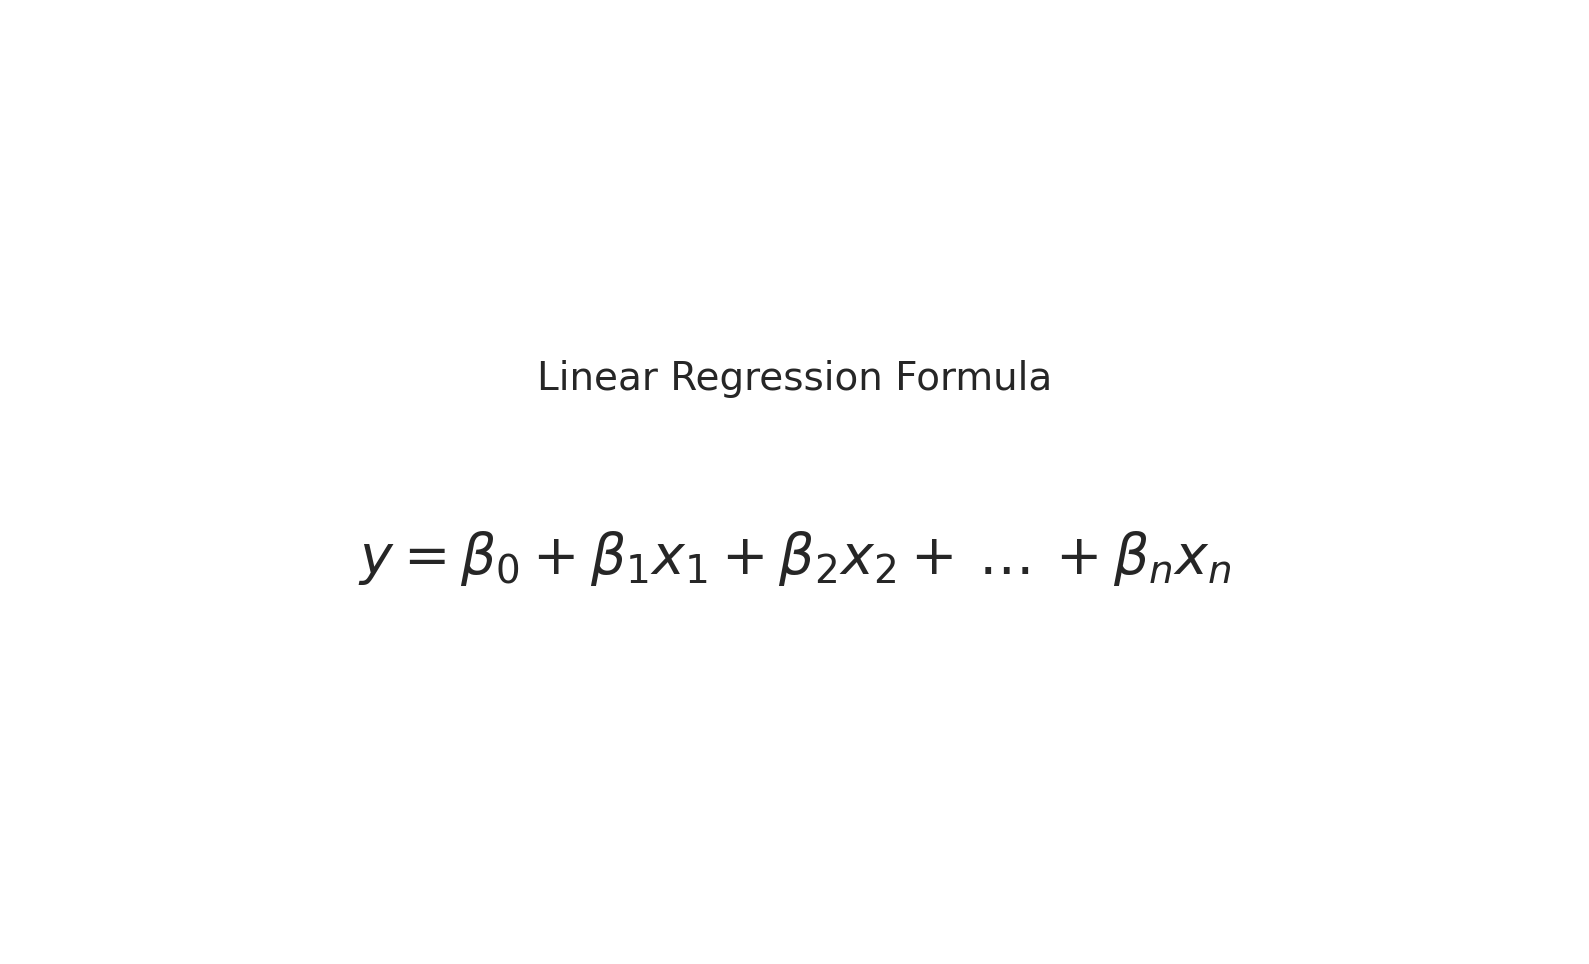
\includegraphics[width=0.9\linewidth]{model_formula_explained.png}
    \caption{Linear regression model components}
  \end{figure}
\end{frame}

\begin{frame}{Results}
  The model produced an intercept of \texttt{53.217}. The coefficient for test preparation was \texttt{5.87}, indicating a positive impact. Lunch type and Race/Ethnicity type E also had significant positive coefficients.
\end{frame}

\begin{frame}{Visuals: Results}
  \begin{figure}
    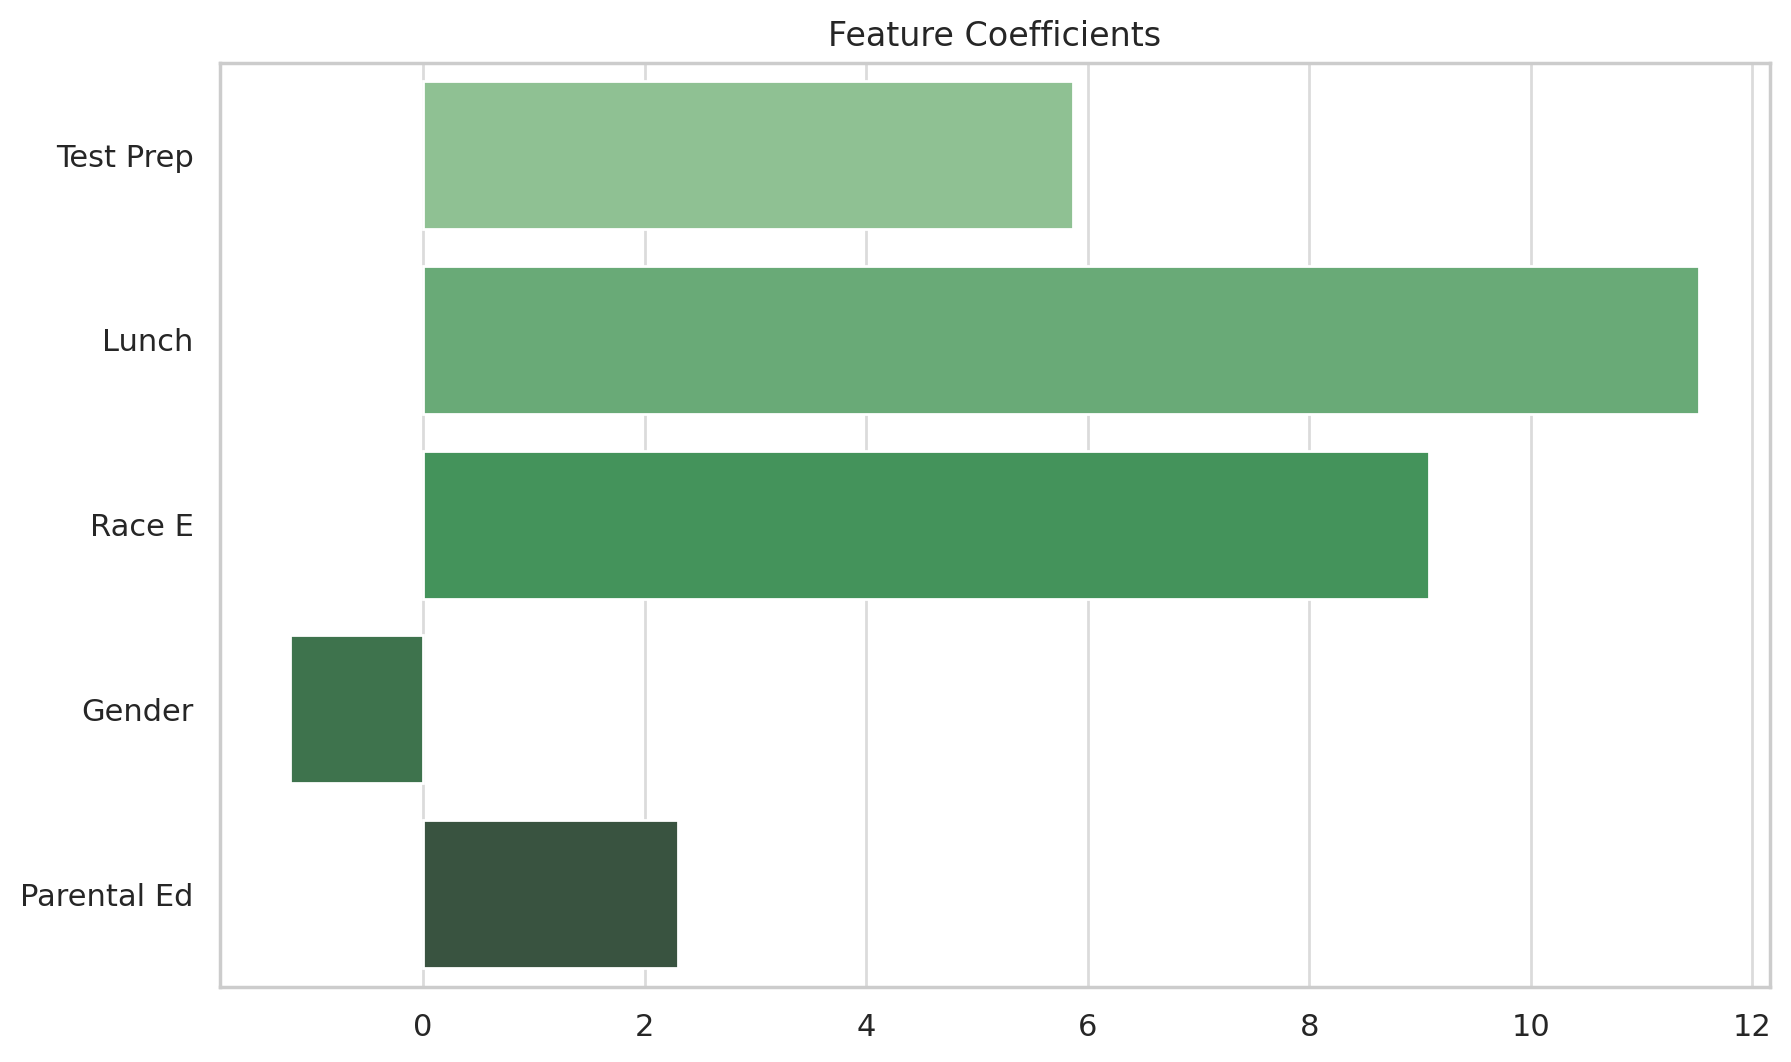
\includegraphics[width=0.9\linewidth]{feature_coefficients.png}
    \caption{Bar chart of feature coefficients}
  \end{figure}
\end{frame}

\begin{frame}{Interpreting the Results}
  The test preparation coefficient of 5.87 suggests that students who completed test prep scored nearly 6 points higher. Lunch type (\texttt{11.52}) may reflect broader socioeconomic advantages. Race/Ethnicity group E (\texttt{9.08}) also showed higher scores.
\end{frame}

\begin{frame}{Visuals: Interpreting the Results}
  \begin{figure}
    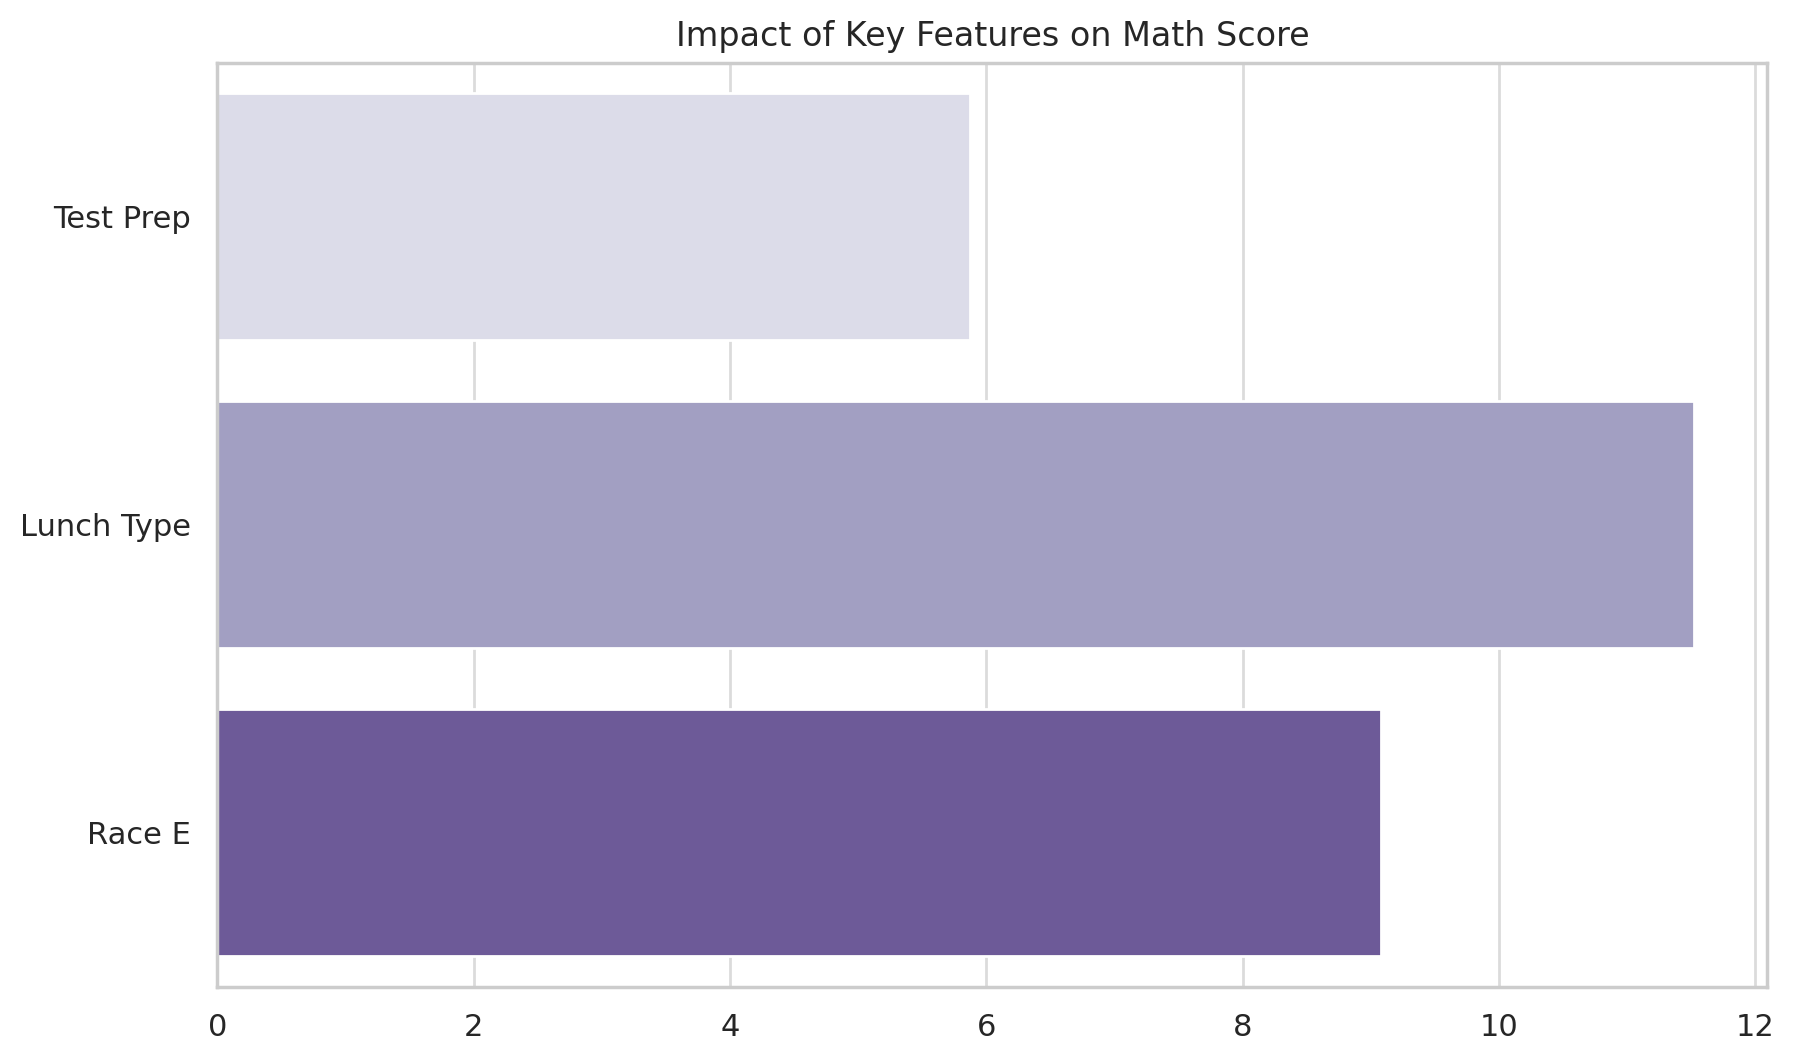
\includegraphics[width=0.9\linewidth]{impact_summary_chart.png}
    \caption{Interpreting key feature impacts}
  \end{figure}
\end{frame}

\begin{frame}{Model Evaluation}
  The model's Mean Squared Error was approximately 200, with a Root Mean Squared Error (RMSE) of 14.1. This implies that predictions deviate by about 14 points on average.
\end{frame}

\begin{frame}{Visuals: Model Evaluation}
  \begin{figure}
    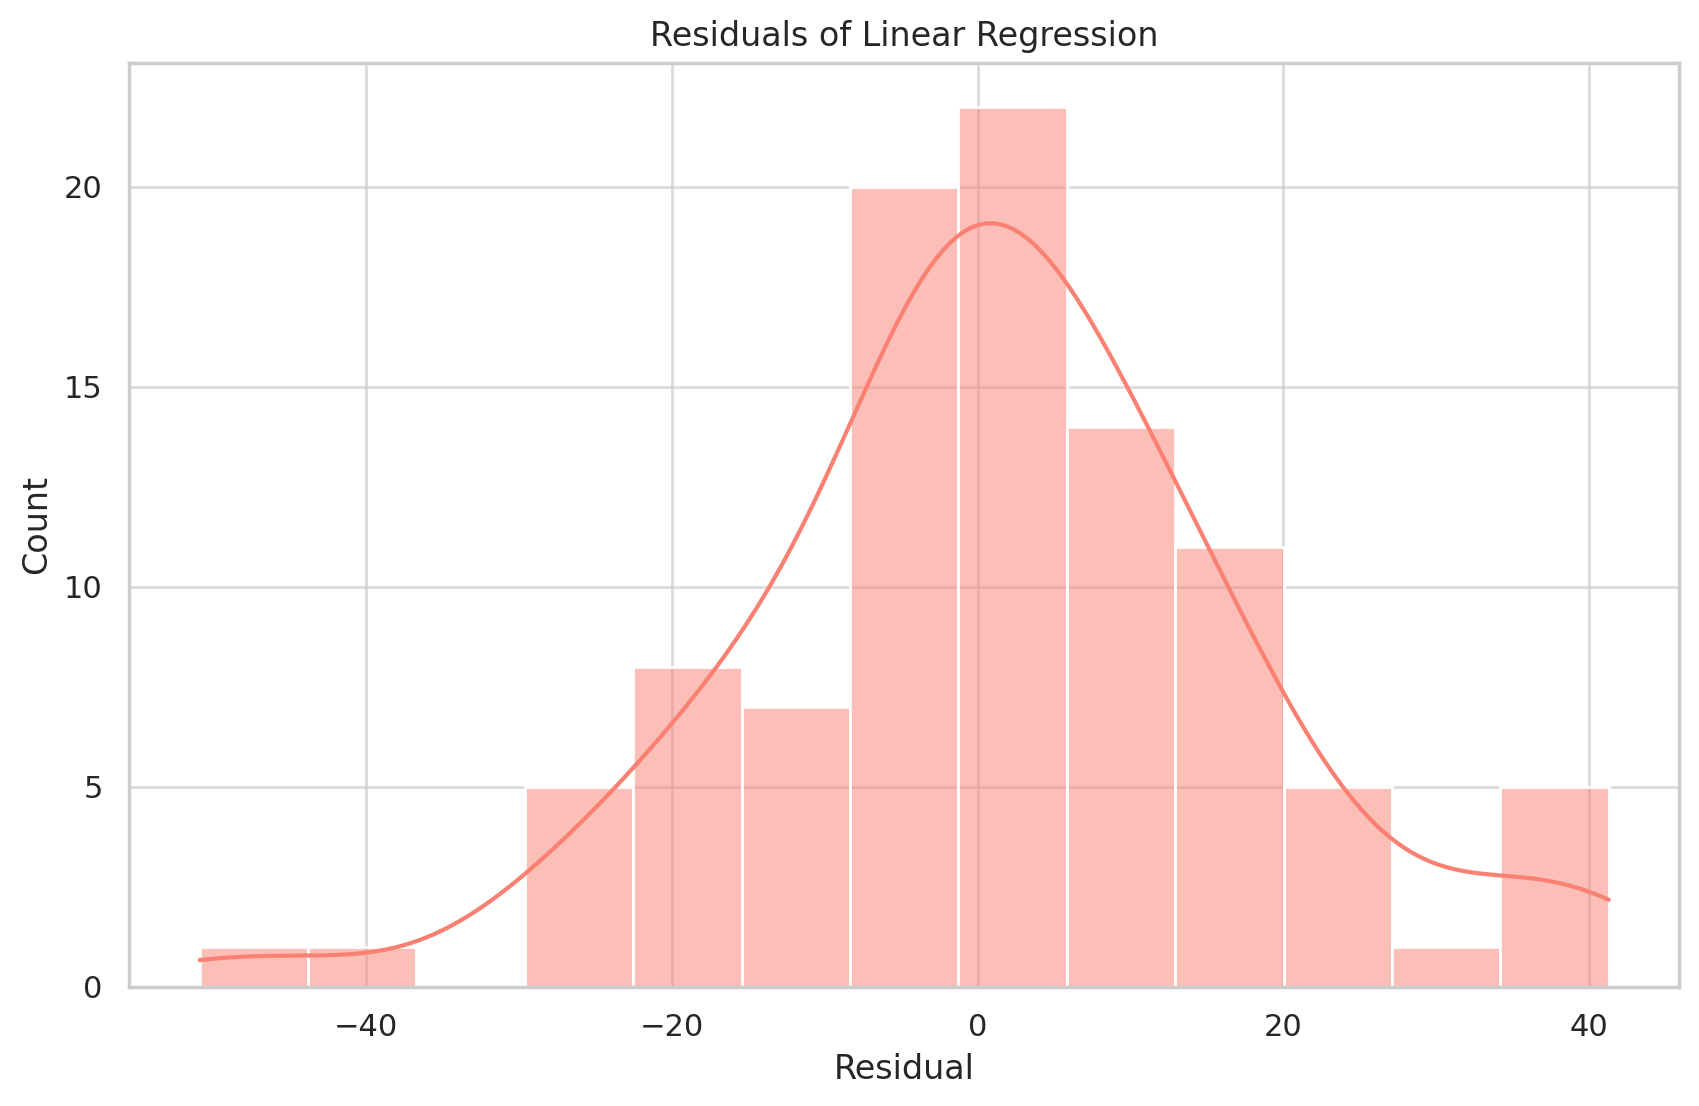
\includegraphics[width=0.9\linewidth]{residuals_plot.png}
    \caption{Residuals plot for linear regression}
  \end{figure}
\end{frame}

\begin{frame}{Random Forest Evaluation}
  We implemented a Random Forest Regressor with Grid Search and cross-validation. Despite its complexity, the RMSE was 14.8—slightly higher than linear regression. This suggests the relationships in the data are mostly linear.
\end{frame}

\begin{frame}{Visuals: Random Forest Evaluation}
  \begin{figure}
    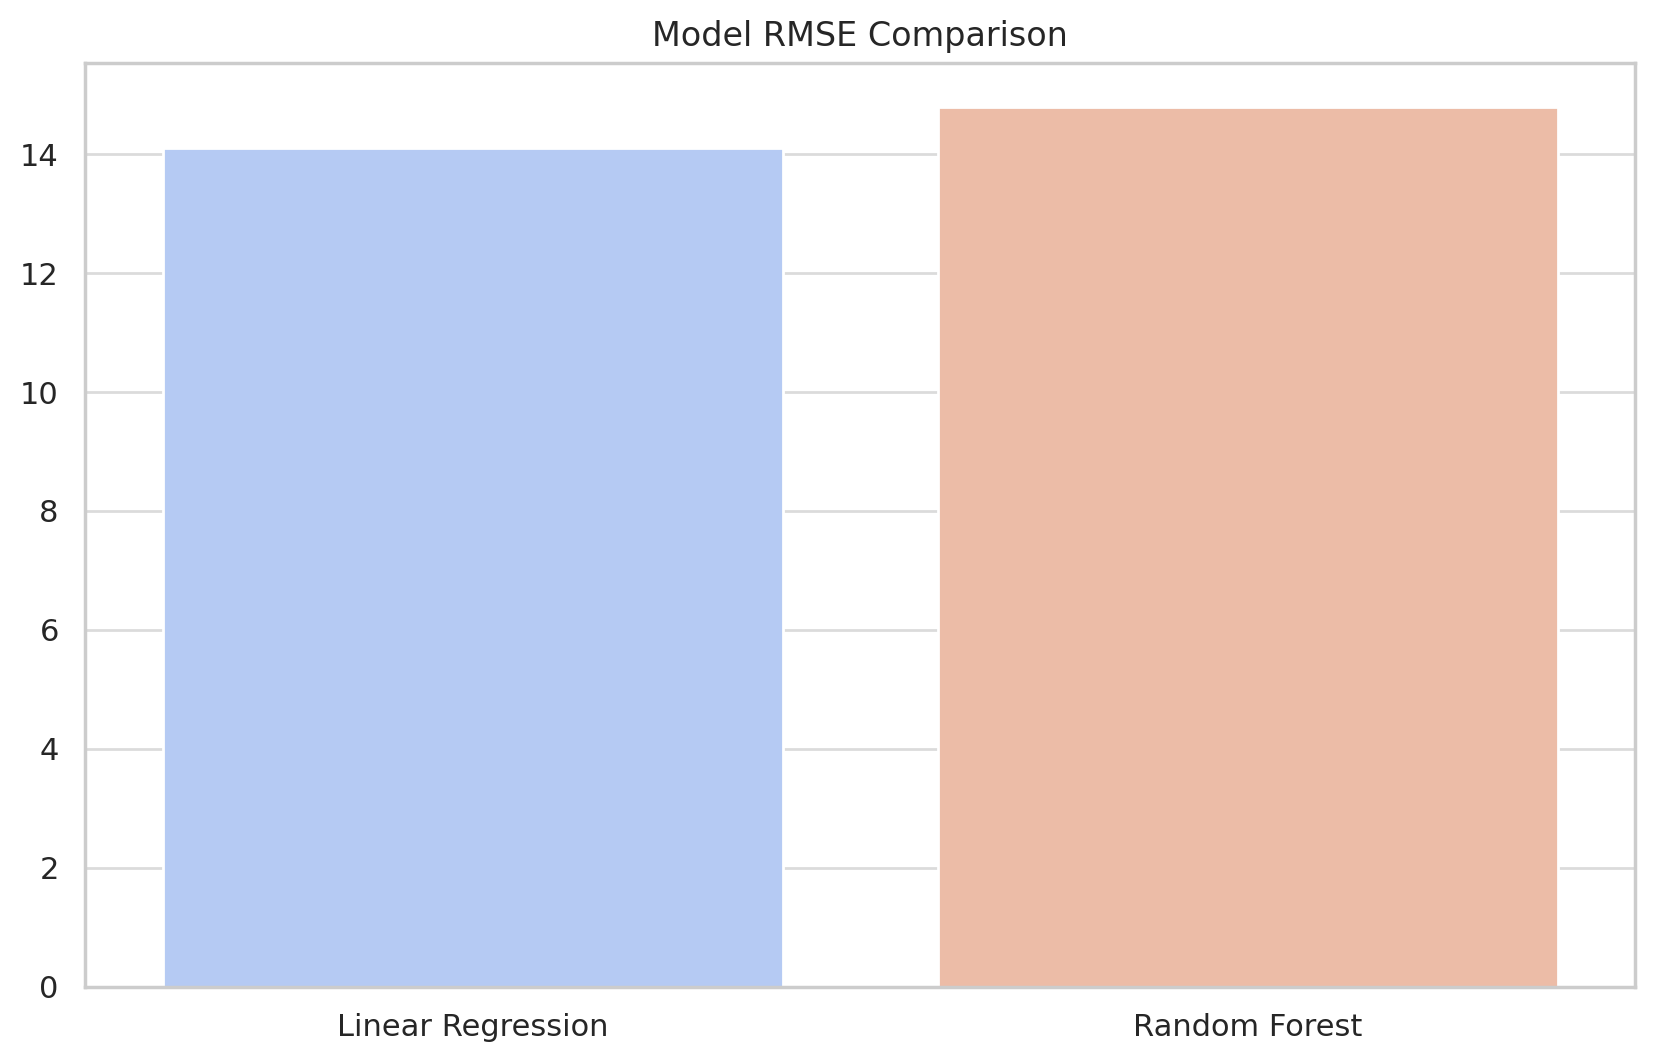
\includegraphics[width=0.9\linewidth]{random_forest_performance.png}
    \caption{Random Forest vs Linear Regression comparison}
  \end{figure}
\end{frame}

\begin{frame}{Analysis of the Results}
  Random Forest's similar performance confirms that the dataset likely lacks complex nonlinear relationships. Linear models, being simpler, performed just as well if not better, especially with a relatively small dataset.
\end{frame}

\begin{frame}{Visuals: Analysis of the Results}
  \begin{figure}
    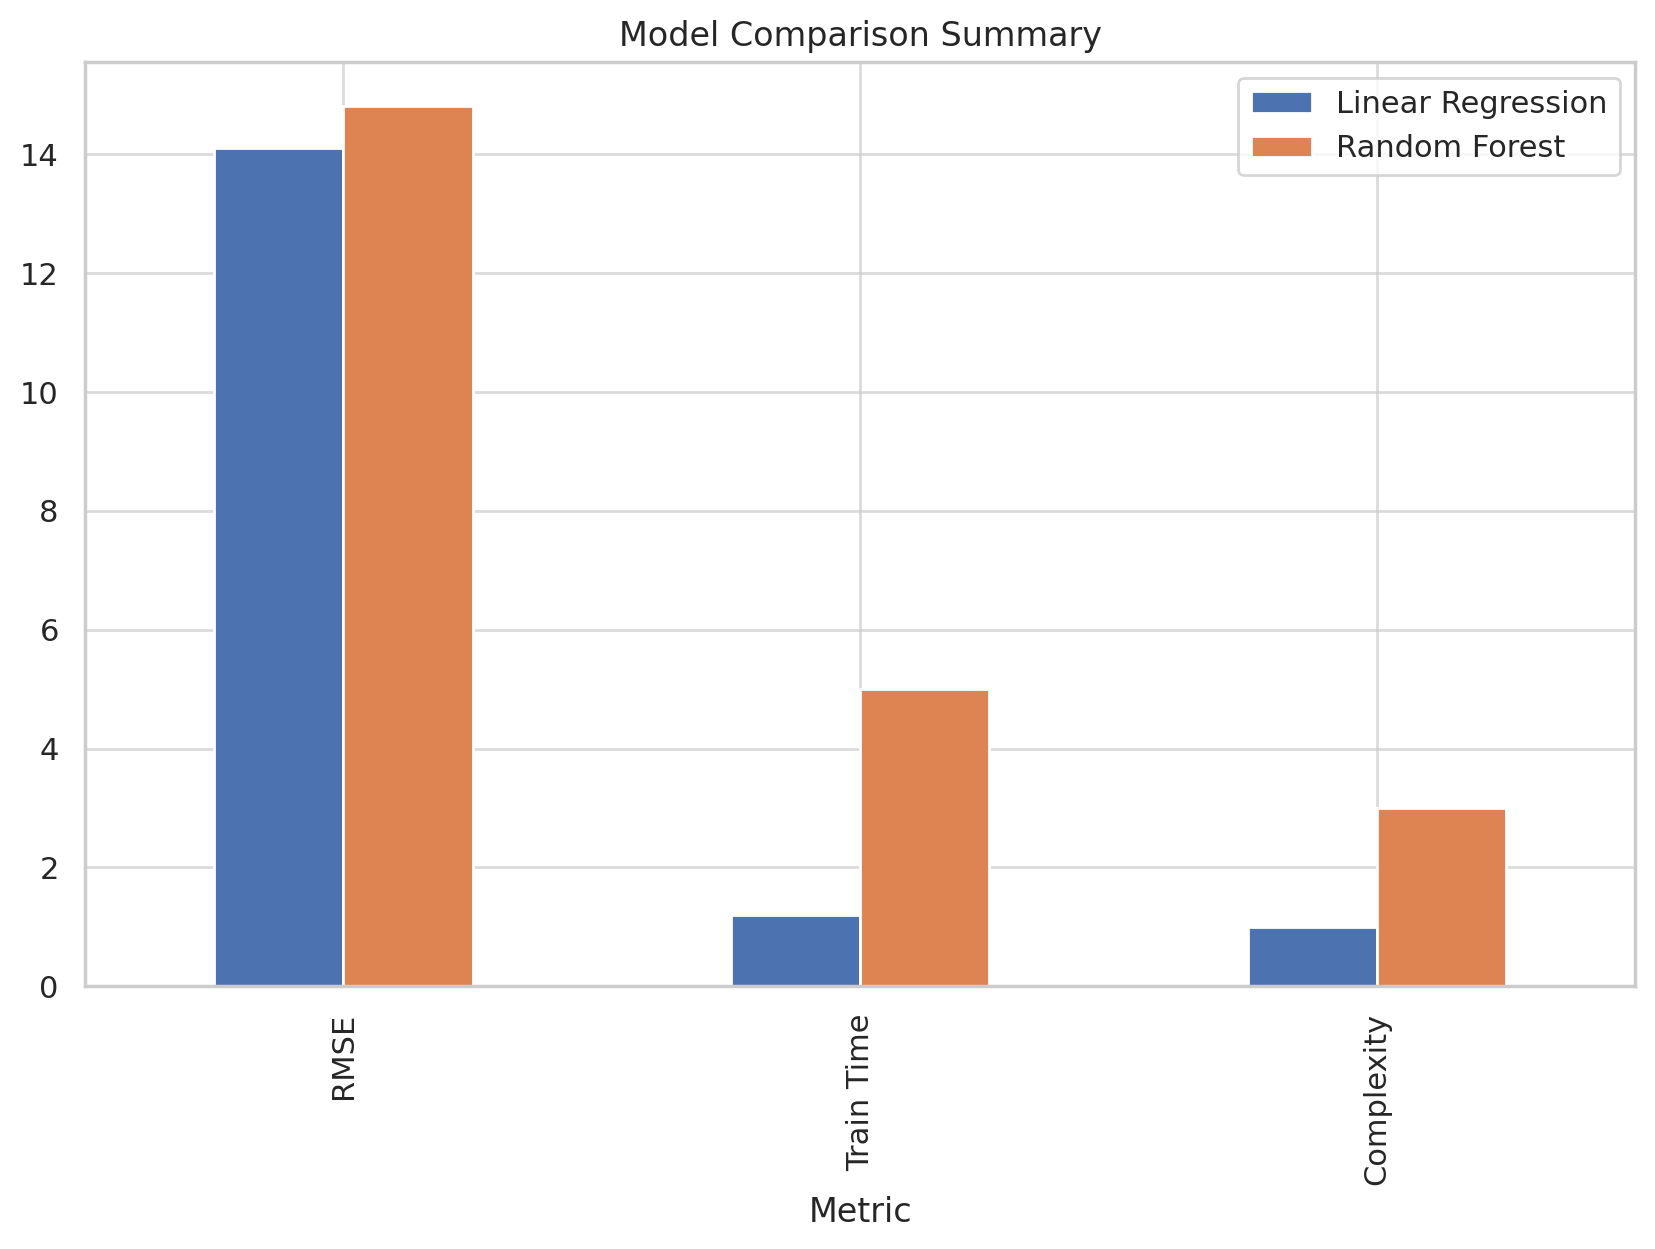
\includegraphics[width=0.9\linewidth]{model_comparison_chart.png}
    \caption{Comparative analysis of model performance}
  \end{figure}
\end{frame}

\begin{frame}{Limitations}
  The model assumes linearity and doesn't account for interactions between features. Factors like personal motivation or home environment are not included but could be impactful.
\end{frame}

\begin{frame}{Conclusion}
  Test preparation, lunch type, and race/ethnicity are influential factors. The linear regression model showed reasonable predictive power, confirming that even simple models can yield valuable insights.
\end{frame}

\begin{frame}{Next Steps}
  Future work includes modeling reading and writing scores, testing interaction effects, and trying ensemble or neural network models for possible performance gains.
\end{frame}

\begin{frame}{Sources}
  \begin{itemize}
    \item Fu, Derek. "AI1 Final Project." Jupyter Notebook, Derek Fu, 27 May 2025.
    \item Seshapanpu, Jakki. “Students Performance in Exams.” Kaggle, 25 July 2018, \href{https://www.kaggle.com/datasets/spscientist/students-performance-in-exams}{https://www.kaggle.com/datasets/spscientist/students-performance-in-exams}.
  \end{itemize}
\end{frame}

\begin{frame}{Acknowledgments}
  I would like to thank Daniel Kim, my AI 1 instructor (as well as my Python 1, 2, and 3 instructor), for his invaluable support throughout the creation of this project.
\end{frame}

\end{document}
